%cSpell:disable
%\documentclass{article}
%\usepackage[margin=0in,paperheight=3.9in,paperwidth=6.3in]{geometry}
%\usepackage[dvipsnames]{xcolor}
%\usepackage{pgfplots}
%\pgfplotsset{width=30cm,compat=1.9}
%\usetikzlibrary{patterns}

%\begin{document}
\begin{figure}[!htb]
  \caption{ROC graph} \label{fig:ROCCurve}
  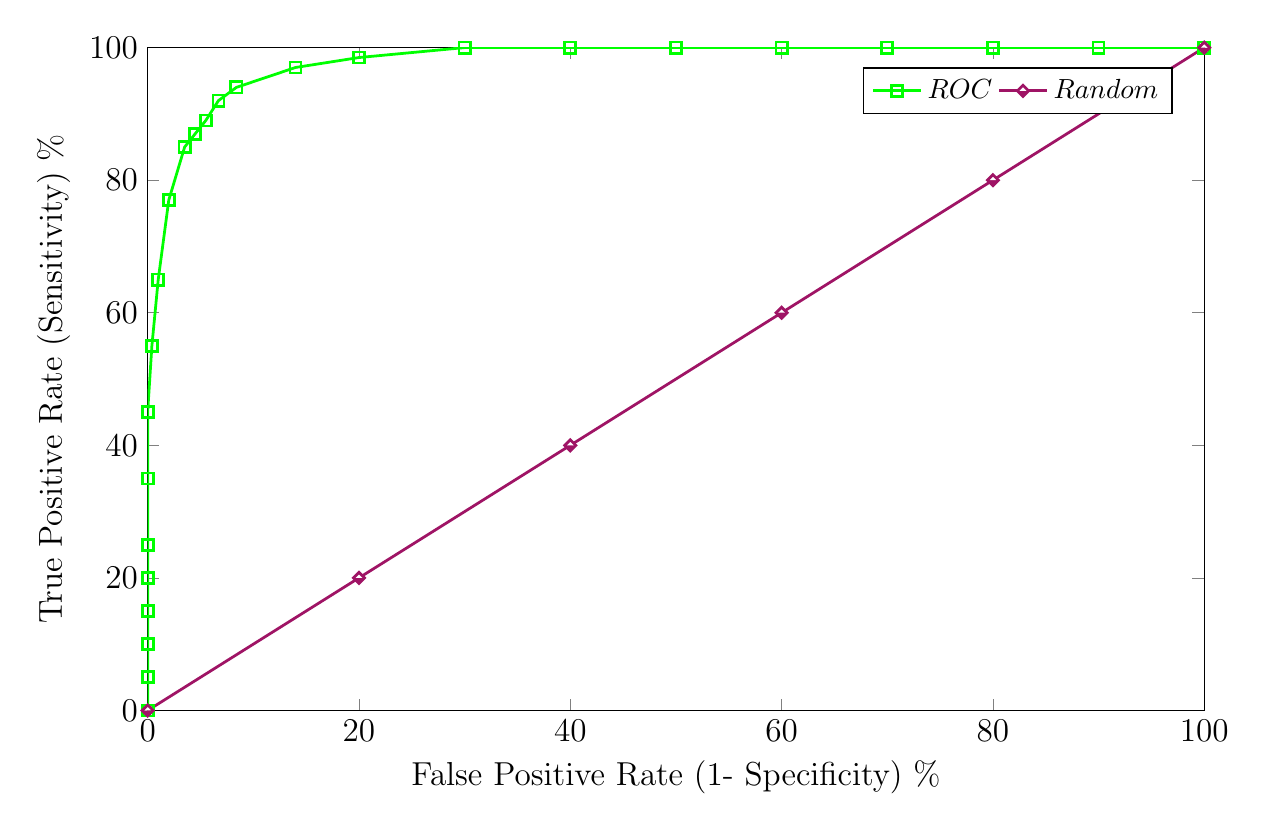
\begin{tikzpicture}
    \begin{axis}
      [
        xlabel={False Positive Rate  (1- Specificity) \%}, ylabel={True Positive Rate (Sensitivity) \%}, xmin=0.0, xmax=100,
        ymin=0.0, ymax=100,
        height=10cm,
        width=15cm,
        legend columns=5,
        legend pos=north east,
        ticklabel style = {font=\large},
        label style = {font=\large},
        xtick={0, 20, 40, 60, 80, 100},
        ytick={0, 20, 40, 60, 80, 100},
      ]

      \addplot
      [
        line width=1pt,
        color=green,
        mark=square,
      ]
      coordinates{
          (0.0, 0.0) (0.0, 5) (0.0, 10) (0.0, 15) (0.0, 20) (0.0, 25) (0.0, 35) (0.0, 45) (0.4, 55) (1, 65) (2, 77) (3.5, 85) (4.5, 87)
          (5.5, 89)  (6.7, 92) (8.4, 94) (14, 97)
          (20, 98.5) (30, 100) (40, 100) (50, 100) (60, 100) (70, 100) (80, 100) (90, 100) (100, 100)};

      \addplot
      [
        line width=1pt,
        color=RedViolet,
        mark=halfsquare*,
      ]
      coordinates{
          (0.0, 0.0) (20, 20) (40, 40) (60, 60) (80, 80) (100, 100) };

      \legend{$ROC$,$Random$}
    \end{axis}
  \end{tikzpicture}

  \begin{align*}
    True Positive Rate  & = \frac{TP}{(TP+FN)} \\
    False Positive Rate & = \frac{FP}{(TP+FN)} \\
  \end{align*}

\end{figure}

%\end{document}
%cSpell:enable